One of the most important things when optimizing CUDA code, is optimizing the memory access done by the kernel which is being executed. The CUDA GPU memory model, which is described in depth in \cref{sec-hw-memory-mode}, contains five levels of memory going from smallest and fastest to largest and slowest, \texttt{Registers}, \texttt{Shared Memory}, \texttt{Level 1 Cache}, \texttt{Level 2 Cache} and \texttt{Global Memory}. While all of these should be kept in mind, while optimizing a CUDA program, it can be seen in \cref{sec-pm-memory} in the chapter describing the programming model, that when programming, there is only four type of memory to be concerned with, \texttt{Host Memory}, \text{Global Memory}, \text{Shared Memory} and \texttt{Local Memory}.\\
To understand how these levels of memory can be used to improve performance, another topic which was also discussed earlier needs to be accounted for. The subject here is Warps, discussed in \cref{sec-hw-warps}. When threads get divided into Warps in each streaming multiprocessor, the device attempts to issue global memory access into as few transactions as possible to minimize DRAM bandwidth. The goal here is to access coalesced memory. Here the interpretation of coalesced memory is "combine (elements) in a mass or whole"//TODO REF. Where the indication for the memory here is that coalesced memory is memory which is closely related, and placed next to each other when look at the address space of the memory. This in turn means that to optimize memory access, we have to have treads access memory, which is beside each other in the memory address space, this is often only the case when a warp contains a large number of threads.\\

\begin{figure}[ht]
	\centering
	\fbox{
		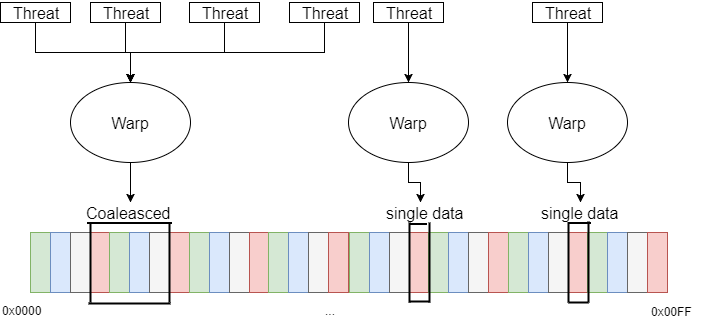
\includegraphics[width=0.9\textwidth]{figs/opti/coalesed_memory.png}
	}
	\caption{Example of coalesced memory access vs random memory access}
	\label{fig:coalesced_memory}
\end{figure}

\Cref{fig:coalesced_memory} show how multiple threads being in the same warp, accesses coalesced memory. The reason for coalesced memory being important is that single data access is often just as expensive in time as it is to access larger pieces of data. This is because memory is only read in chunks, which correlates to a single read being able to supply multiple threads with data or a single threat with a large amount of data of which there is no guarantee that it uses all of.\\

However, it is very difficult to avoid all random memory access, which is where our memory model become important, as different levels of memory is available for use. Instead of using the slower \texttt{Global memory}, \texttt{Shared memory} can be used for the random memory access. This can be accomplished by using shared memory as a buffer.